% figures-es/signal-quality.tex
% Standalone TikZ: la jerarquía de señales de conversión (ch.10). Más ancho = alto volumen /
% bajo valor (clic); más estrecho = bajo volumen / alto valor (cerrado-ganado).
\documentclass[tikz,border=4pt]{standalone}
\usepackage{tikz}
\usetikzlibrary{arrows.meta,positioning}

\definecolor{s1}{HTML}{9AA7B0}
\definecolor{s2}{HTML}{5E8597}
\definecolor{s3}{HTML}{0E6655}
\definecolor{s4}{HTML}{16557A}
\definecolor{s5}{HTML}{1A5276}

\begin{document}
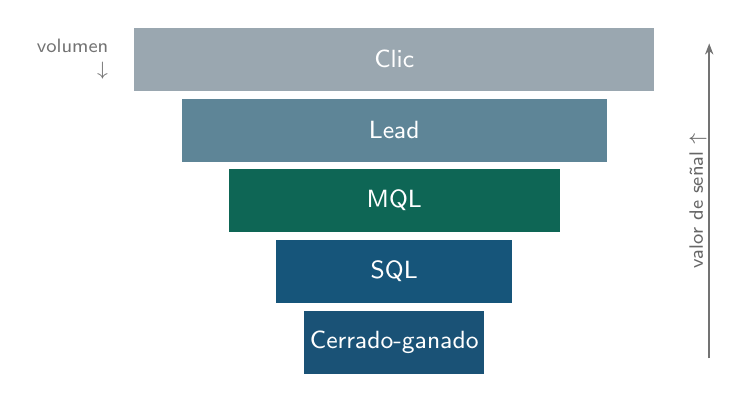
\begin{tikzpicture}[
  band/.style={draw=none, fill=#1, text=white, font=\sffamily\small,
               minimum height=8mm, align=center, inner sep=2pt},
]
  \node[band=s1, minimum width=66mm] (b1) at (0,0)     {Clic};
  \node[band=s2, minimum width=54mm] (b2) at (0,-9mm)  {Lead};
  \node[band=s3, minimum width=42mm] (b3) at (0,-18mm) {MQL};
  \node[band=s4, minimum width=30mm] (b4) at (0,-27mm) {SQL};
  \node[band=s5, minimum width=18mm] (b5) at (0,-36mm) {Cerrado-ganado};

  % flecha de valor ascendente a la derecha
  \draw[-{Stealth[length=4pt]}, black!55, line width=0.8pt] (40mm,-38mm) -- (40mm,2mm)
    node[midway, right=1mm, font=\scriptsize\sffamily, text=black!60, rotate=90, anchor=south] {valor de señal $\uparrow$};
  % nota de volumen descendente a la izquierda
  \node[left=2mm of b1, font=\scriptsize\sffamily, text=black!55, align=right] {volumen\\$\downarrow$};
\end{tikzpicture}
\end{document}
